%!TEX root = ../main.tex
\chapter{基于情感词典的情感分析}
在情感分析领域,情感词典在早期的研究中有着重要地位,对提升分类效果有着很大帮助。基于情感词典的情感分类技术主要是利用句中每个情感词的情感值,进行加权累加得出整句情感得分,最后根据情感得分来划分情感极性。情感词典技术的一大弊端在于,如果情感词典的规模不够大,对于情感词的覆盖面不够广,对情感分析的帮助有限。本章基于多种情感词典,结合出一个规模相对较大的情感词典,在实验结果上表现良好,证明扩大情感词典规模对提升情感分类效果有着很大帮助。

\section{情感词典构建}\label{section:情感词典构建}
我们利用互联网上的各种开源中文情感字典,结合一些辅助情感字典,再进行针对本文特定数据集,构建出用于本文情感分析的情感字典。

\subsection{基础情感词典构建}
在基础情感字典上,我们选取中文自然语言处理常用的三个情感字典,包括:知网情感字典(HowNet)\cite{hownet},台湾大学开发的简体中文情感极性词典(NTUSD)\cite{NTU}和清华大学李军\cite{li2007experimental}开发的中文褒贬义词典。在对三个词典进行交叉去重后,我们发现,有的词典中的积极词汇在别的词典中则被标记为消极。因此我们选用一种根据情感极性和词典权威度的投票筛选来确定这些词的情感极性\cite{_hownet_2008},公式如下:

\begin{equation}
\operatorname{Polarity}=\left\{\begin{array}{cc}
-1, &{\sum P(w) \leq-1}\\
0,  &{others}\\
+1, &{\sum P(w) \geq 1}
\end{array}\right.
\end{equation}
如果是属于others的情况,则根据词典权威度(HowNet > NTUSD > 中文褒贬义词典)来决定该词的情感极性。最终我们构建出基础情感词典的雏形,共含11,189个积极词汇,15,288个消极词汇。

在上面构建好的词典雏形的基础上,我们继续丰富基础情感词典,使用的词典如下:

\begin{enumerate}[(1)]
\item 程度词词典

中文中常在情感词前来增加或削弱该情感词的情感强度,这类词对分析文本情感倾向有着重要意义,因此,我们建立了一种包含六类程度词的词典,部分程度词及其对情感词的加成系数如下\tabref{chengduci}:
\begin{table}[htbp]
\begin{center}
\caption{程度词词典及其加成系数表}
\label{tab:chengduci}
\begin{tabularx}{\linewidth}{ZZZZ}\toprule
程度 & 加成系数 & 示例 & 个数 \\\midrule
极其/most & 2 & 绝对、完全、异常 & 89\\
很/very & 1.75 & 不少、出奇、很 & 88\\
较/more & 1.5 & 更、还、比较 & 46\\
稍/ish & 1.25 & 略、挺、有点 & 42\\
微/insufficiently & 0.8 & 不怎么、丝毫、微 & 12\\
超/over & 0.6 & 超、过、过于 & 30\\\bottomrule
\end{tabularx}
\end{center}
\end{table}

\item 否定词词典

否定词其实是一种特殊的程度词,它可以将整个词的情感极性反转,对于否定词的加成系数,取决于情感词前的否定词个数,若是偶数,则为1,即双重否定为肯定;若是奇数,则为-1。我们选用了常见的24个否定词,包括不是、没、无、非、不曾、绝不等。

\item 连接词词典

在中文中常有一些可以影响句子整体上的情感的连接词。比如:他虽然很帅,但是人品很差。如果忽略连接词的作用,	``很帅''和``很差''的情感倾向相互抵消,整句话就会被判定为中性,但是实际情感更倾向于消极。因此,不能忽视连接词对整句话情感倾向影响,所以我们引入了连接词词典,部分连接词和其加成系数如下\tabref{lianjieci}:
\begin{table}[htbp]
\caption{连接词和其加成系数表}
\label{tab:lianjieci}
\begin{tabularx}{\linewidth}{ZZZZ}\toprule
属性 & 加成系数 & 示例 & 个数 \\\midrule
让步 & 1.2 & 不过、虽然、不料 & 9\\
递进 & 1.5 & 也、其次、不仅 & 5\\
因果 & 2 & 但是、况且、然而 & 10\\
转折 & 3 & 甚至、尤其、居然 & 3\\\bottomrule
\end{tabularx}
\end{table}

\item 停用词词典

在进行分词处理后,每个句子都变成一串词组成的列表,除去文本预处理时已经完成的工作,添加停用词词典能更好的进行文本情感分析,并且提高处理速度。我们设置的停用词词典为哈尔滨工业大学发表的停用词词表。

\end{enumerate}

\subsection{基础情感词典的扩展}
在完成上述工作后,我们发现情感词典的包含的情感词数量已经足够,但仍需要对本文所用的数据集进行针对性添加。因此我们添加了包含网络用语的针对微博语境的情感词典和微博情感词典。

在基础情感词典中已经包含了日常生活中常出现的情感词,但是微博作为社交网络,拥有着大量网络用语,新兴词汇和非标准简称,如果不能有效的判断出这些词汇的情感词属性和情感极性,会影响情感分类的准确性。因此我们添加了开源情感词典:BosonNLP\cite{boson},该词典包含114,767条词汇,极大的丰富了情感词典的内容。

用户在微博上发表的文本往往并非纯文字,而是包含各种表情符号的文本,而这些表情符号也包含着丰富的情感信息\cite{中文微博情感分析},添加微博表情符号词典能有效帮助我们进行情感分析。我们选用微博上常用的20个表情添加到表情符号词典中,其中积极和消极各10个,具体表情符号如下\tabref{biaoqing}:
\begin{table}[htbp]
\begin{center}
\caption{表情符号词典}
\label{tab:biaoqing}
\begin{tabularx}{\linewidth}{ZZZ}\toprule
情感 & 示例 & 个数 \\\midrule
积极 & [可爱]、[太开心]、[嘻嘻]& 10\\
消极 & [怒]、[衰]、[骷髅]& 10\\\bottomrule
\end{tabularx}
\end{center}
\end{table}

\section{基于情感词典的情感分析过程}
上一节中,我们提出了如何构建基础情感词典,并针对数据集,有目的性的对基础情感词典进行扩充。下面详细解释如何将构建好的情感词典用于情感分析。主要流程分为三步:1、对文本进行预处理,2、构建情感词典,并设置不同规模的情感词典作为对照组,3、编写代码对数据集进行分析,最后比较训练模型的结果与预先标记好的句子情感极性。流程图见图\ref{fig:情感词典流程图}。文本预处理和情感词典构建的详细过程分别见章节\ref{section:文本预处理}和章节\ref{section:情感词典构建}
\begin{figure}[htbp]
\begin{center}
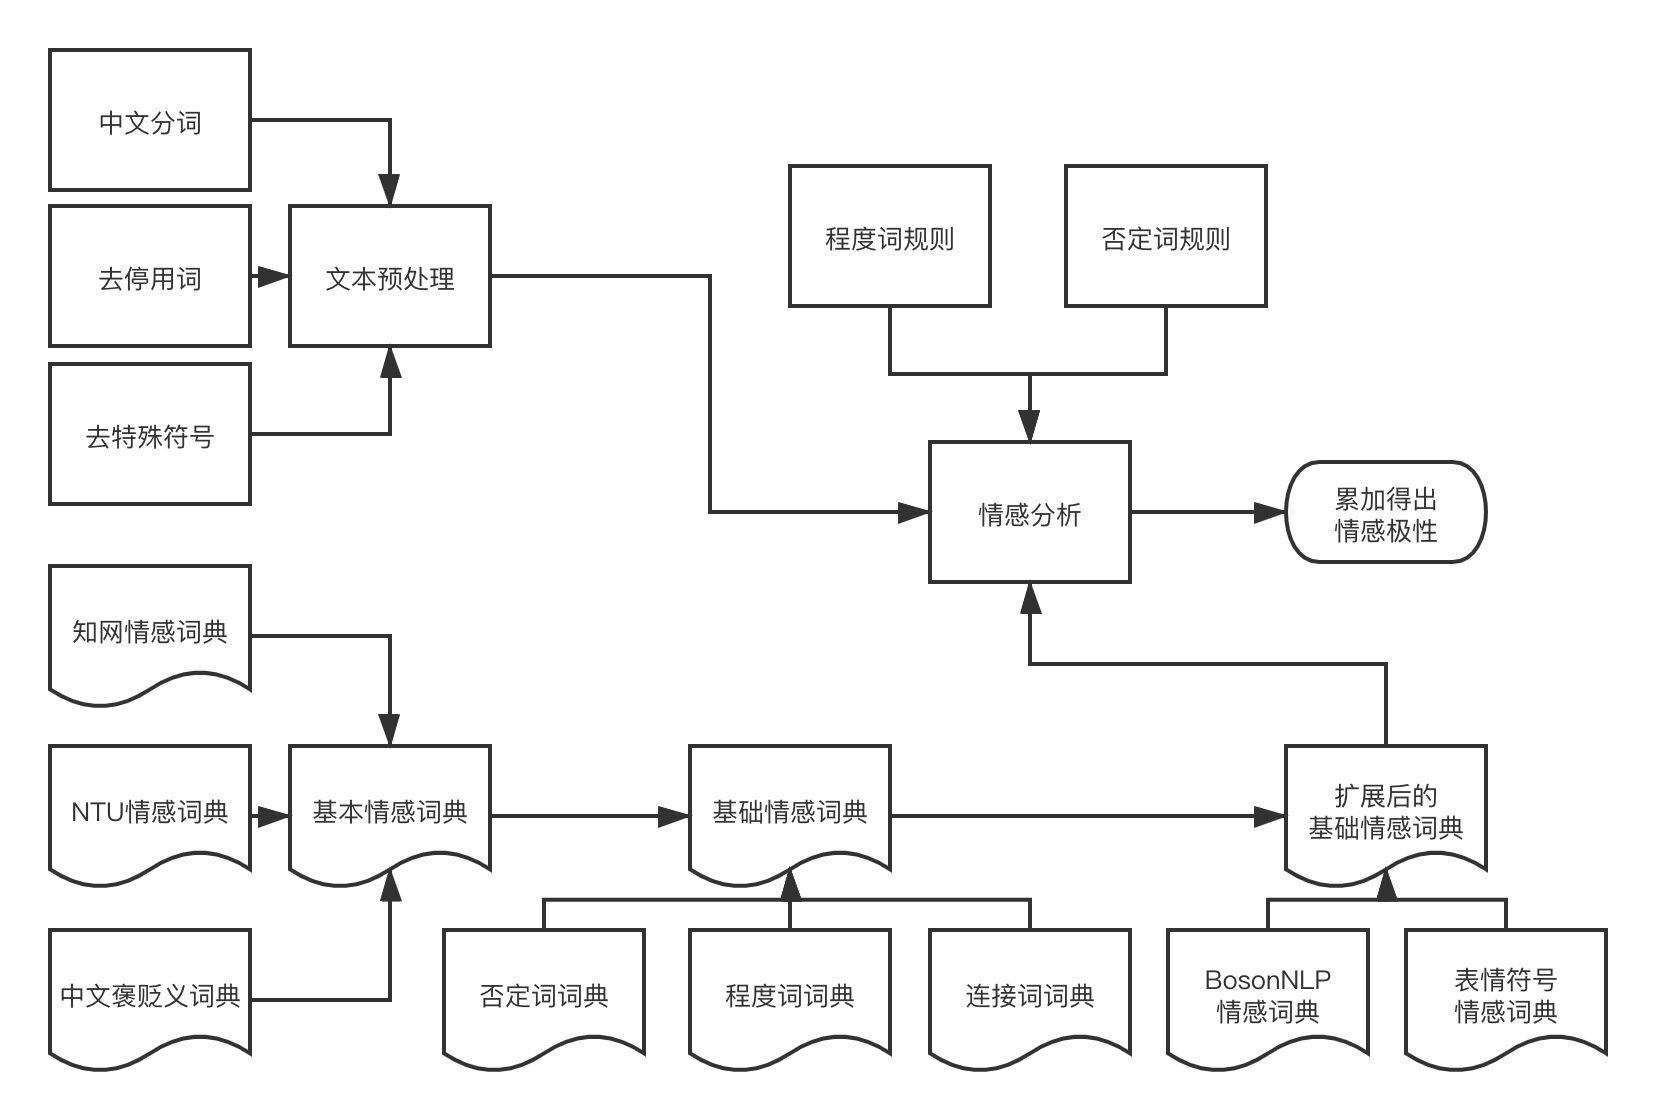
\includegraphics[height=100mm]{情感词典流程图.png}\\
\end{center}
\caption{基于情感词典的情感分析过程流程图}
\label{fig:情感词典流程图}
\end{figure}

在计算整句情感极性时,我们设计了公式\ref{eq:整句情感极性公式},其中$S_{w_{i}}$为该句中第$i$个词的情感值,$p_j$为该词前面连接词/程度词的加成系数。若无连接词/程度词,则${\prod_{j=1}^{m} p_{j}}$默认为1。$d$为该词前面的否定系数,若否定词数量为偶数,则${\prod_{j=1}^{m} d_{j}}$为1,否则为-1。$m$通常取3,若该词前面词数量不足3,则视情况选取(若该词属于句首,则$m$取0)。最后将这句话中每个情感词乘以加成系数和否定系数后的情感值相加,若是大于0,则为积极,否则为消极。

\begin{equation}
\label{eq:整句情感极性公式}
\text { Polarity }_{total}=\left\{\begin{array}{ll}
1, & \sum_{i=1}^{n}\left(S_{w_{i}} \prod_{j=1}^{m} p_{j} d_{j}\right)>0 \\
0, & \sum_{i=1}^{n}\left(S_{w_{i}} \prod_{j=1}^{m} p_{j} d_{j}\right) \leq 0
\end{array}\right.
\end{equation}


\section{实验结果与分析}
本文中使用的数据集为互联网开源的微博数据集,共包含119,988条带标注的微博文本数据。其中积极文本和消极文本各占一半。情感词典包括知网情感词典、台湾大学简体中文情感极性词典、中文褒贬义词典、BosonNLP开源情感词典、哈工大停用词表、自建表情符号情感词典、连接词词典、否定词词典、程度词词典。实验平台运行在Google Colab(Jupyter Notebook)上,编程语言为Python,使用的开源库包括Jieba,Numpy,Pandas等。该实验的情感分析测评指标采用国际通用的四个标准,即准确率(accuracy)、精确率(precision)、召回率(recall)和F1值。

本实验的三个对照组分别为不同规模的情感词典,为方便描述,我们将他们标记为BD,BD-A,BD-AE。分别为基准情感词典(含知网情感词典,台湾大学简体中文情感极性词典,中文褒贬义词典),在基准情感词典上加入连接词词典,否定词词典,程度词词典等,在BD-A的基础上加入扩展情感词典(包括BosonNLP情感词典,表情符号情感词典)。实验结果如表\ref{tab:qinggancidianjieguo}。

\begin{table}[htbp]
\begin{center}
\caption{不同情感词典下的实验结果}
\label{tab:qinggancidianjieguo}
\begin{tabularx}{\linewidth}{ZZZZZ}\toprule
情感词典 & Accuracy & Precision & Recall & F1值 \\\midrule
BD & 69.17\% & 71.58\% & \textbf{66.77\%} & 69.09\% \\
BD-A & 69.28\% & 71.88\% & 66.67\% & 69.18\% \\
BD-AE & \textbf{75.35\%} & \textbf{92.46\%} & 58.24\% & \textbf{71.46\%} \\\bottomrule
\end{tabularx}
\end{center}
\end{table}

从上表\ref{tab:qinggancidianjieguo}结果看出,BD-AE有效的改进了情感分类效果,基本在各项指标上均优于其他数据集,验证了扩大情感词典规模在提升实验表现上的有效性。但是BD-AE在召回率上表现不佳,即在处理消极文本上仍有可提升空间,也显示出了使用情感词典方法处理情感分析问题上的局限性。该方法只是简单的将句中的每个词的情感值加权相加,根据最终整句的情感值来进行分类,没有考虑到句法,语法上的深层语义。即使继续扩大情感词典规模,可能收益也不会很大。相反,更大规模的情感词典意味着在检索上需要消耗更大的计算资源和时间,得不偿失。

\section{本章小结}
本章介绍了构建中文情感词典及基于基础情感词典进行拓展的过程。首先描述了情感词典在情感分析领域的价值,之后进行了基础情感词典的构建和拓展,然后基于不同规模的情感词典设置对照组进行实验。实验结果表明,扩展后的情感词典一定程度上可以有效提升情感分类的效果。

